\documentclass{standalone}
\usepackage{tikz}
\usetikzlibrary{positioning}

\begin{document}

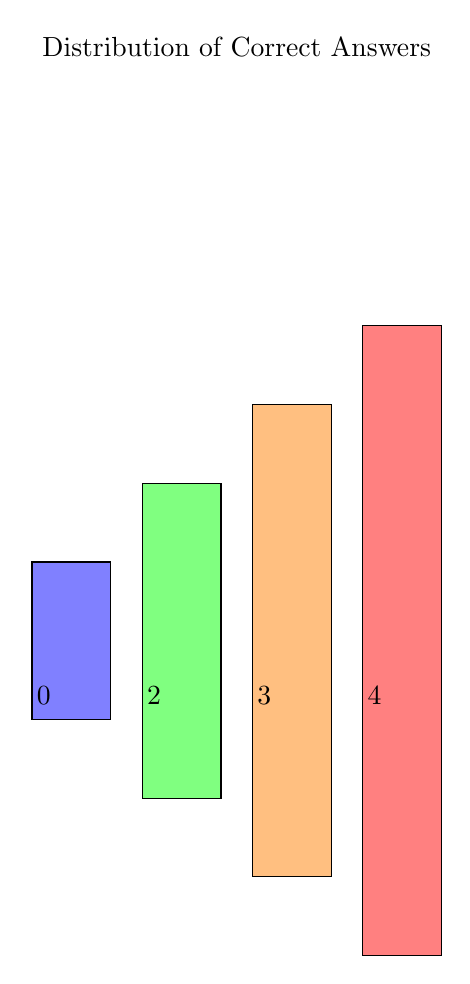
\begin{tikzpicture}[scale=0.7]
    \def\xshift{2cm} % Shift for x-axis labels
    \def\barwidth{1cm} % Width of each bar

    % Define the data points
    \def\noanswers{0}
    \def\twocorrect{2}
    \def\threecorrect{3}
    \def\allcorrect{4}

    % Draw the bars
    \node[draw, fill=blue!50, minimum width=\barwidth, minimum height=2cm] at (\xshift,0) {};
    \node[draw, fill=green!50, minimum width=\barwidth, minimum height=4cm] at (2*\xshift,0) {};
    \node[draw, fill=orange!50, minimum width=\barwidth, minimum height=6cm] at (3*\xshift,0) {};
    \node[draw, fill=red!50, minimum width=\barwidth, minimum height=8cm] at (4*\xshift,0) {};

    % Add labels
    \node at (\xshift - 0.5*\barwidth, -1cm) {\noanswers};
    \node at (2*\xshift - 0.5*\barwidth, -1cm) {\twocorrect};
    \node at (3*\xshift - 0.5*\barwidth, -1cm) {\threecorrect};
    \node at (4*\xshift - 0.5*\barwidth, -1cm) {\allcorrect};

    % Add title
    \node[above=1cm] at (2.5*\xshift, 9cm) {Distribution of Correct Answers};
\end{tikzpicture}

\end{document}